\documentclass[12pt]{amsart}
\usepackage[margin=1in]{geometry}
\usepackage{paralist}

\usepackage{graphicx}
\usepackage{caption}
\usepackage{subcaption}

\theoremstyle{definition}
\newtheorem{question}{Question}

\begin{document}
\begin{center}
\textbf{\Huge
Lesson Plan: Meeting Seven
}
\end{center}
\vspace{.5in}

\section*{Phase 1} Remind students of the nature of Reidemeister moves. Be sure to stress that these are little atomic pieces of ambient isotopies, and very tightly controlled.

Then have them work through a progression of examples:

\begin{figure}[h]
        \centering
        \begin{subfigure}[b]{0.3\textwidth}
                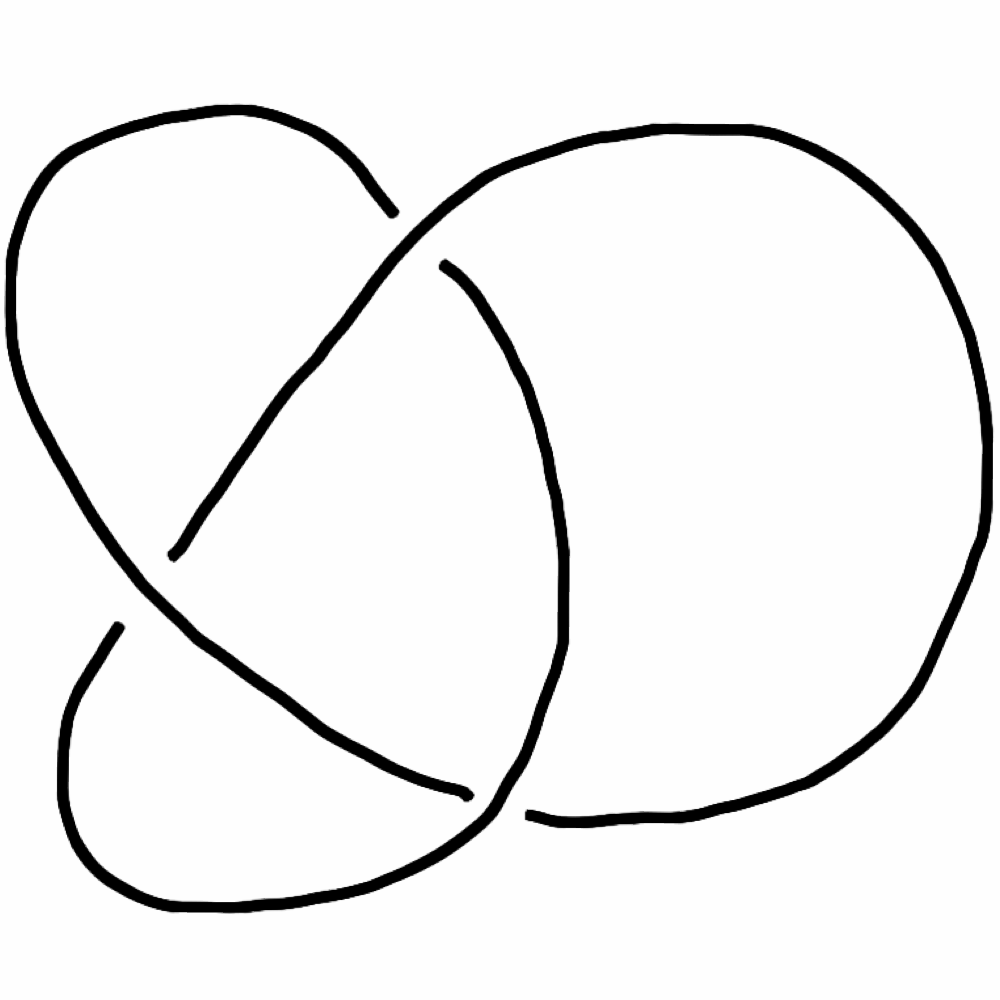
\includegraphics[width=\textwidth]{knotpics/trefoil.png}
                \caption{A trefoil}
        \end{subfigure}
        \begin{subfigure}[b]{0.3\textwidth}
                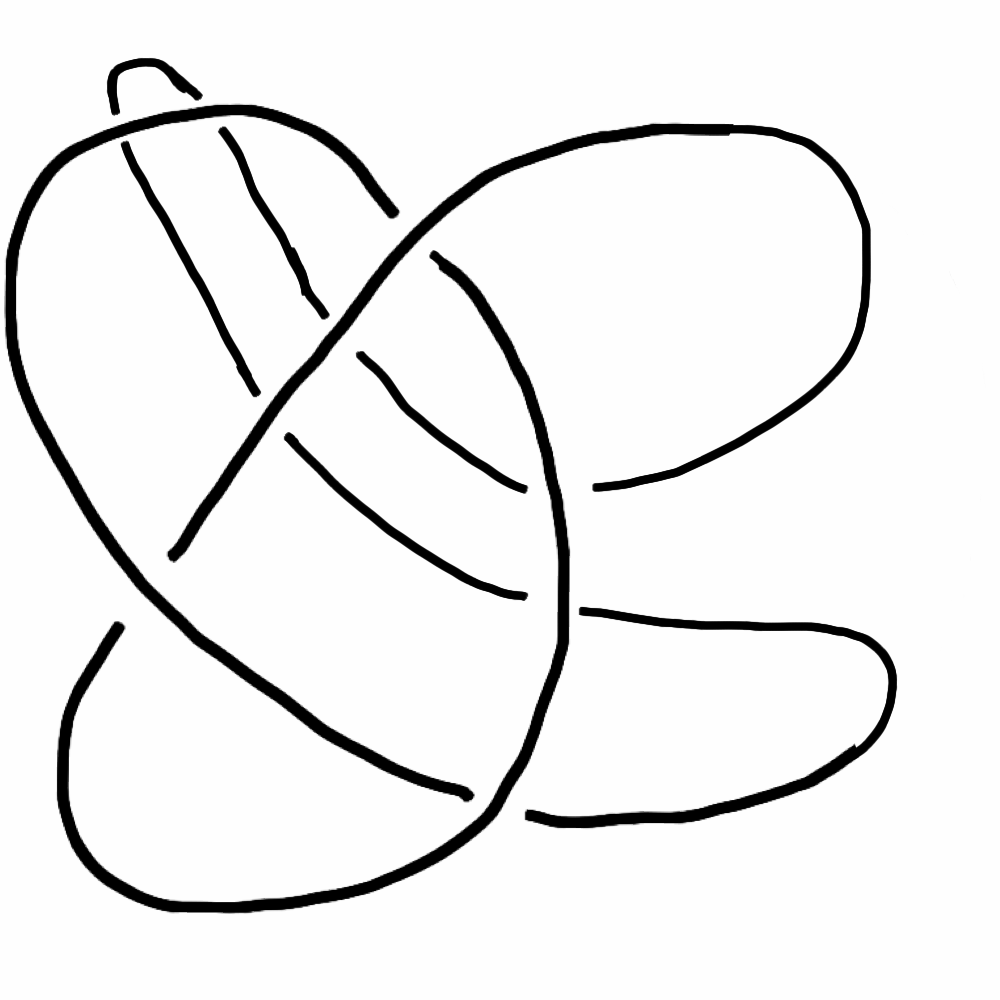
\includegraphics[width=\textwidth]{knotpics/trefoil-wiggled.png}
                \caption{A disguised trefoil}
        \end{subfigure}
\end{figure}

\begin{figure}[h]
        \centering
        \begin{subfigure}[b]{0.3\textwidth}
                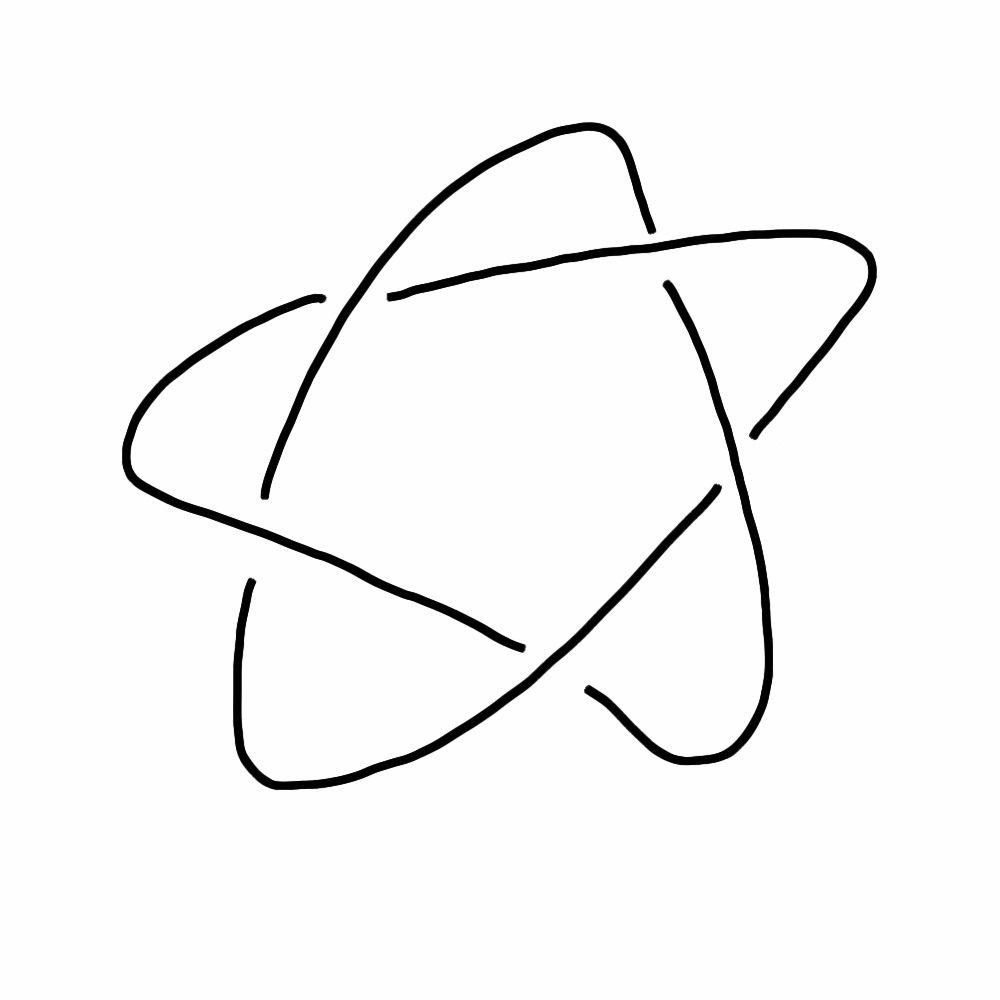
\includegraphics[width=\textwidth]{knotpics/5-1-tj.png}
                \caption{$5_1$}
        \end{subfigure}
        \begin{subfigure}[b]{0.3\textwidth}
                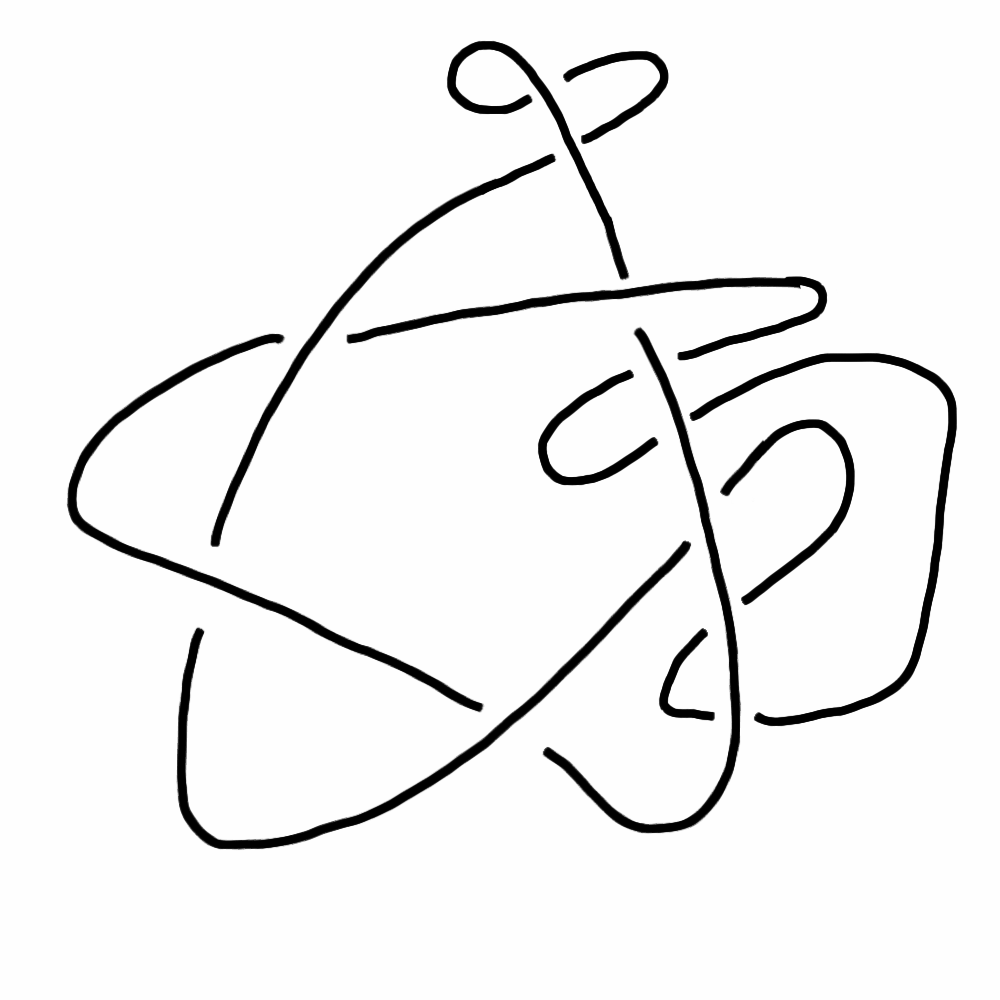
\includegraphics[width=\textwidth]{knotpics/5-1-wiggled.png}
                \caption{A disguised $5_1$}
        \end{subfigure}
\end{figure}

\begin{figure}[h]
        \centering
        \begin{subfigure}[b]{0.3\textwidth}
                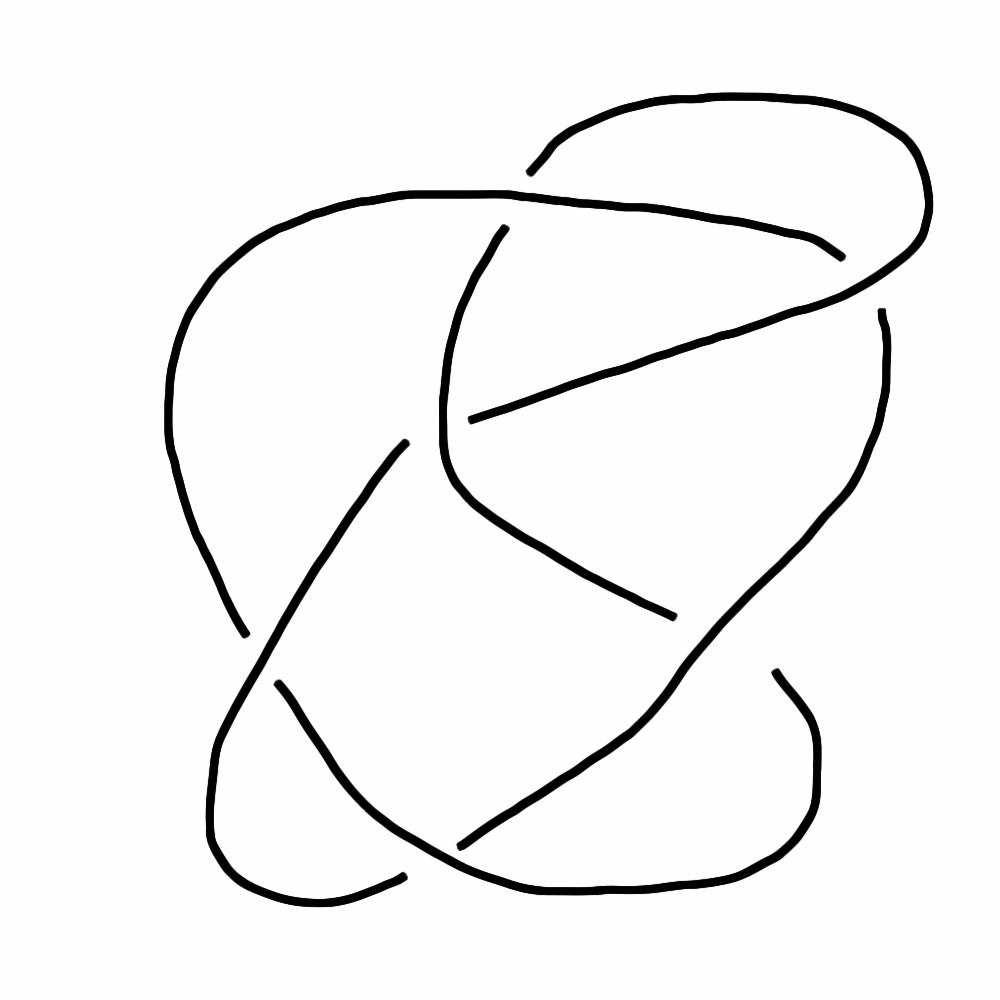
\includegraphics[width=\textwidth]{knotpics/anothersix.png}
                \caption{$6_1$}
        \end{subfigure}
        \begin{subfigure}[b]{0.3\textwidth}
                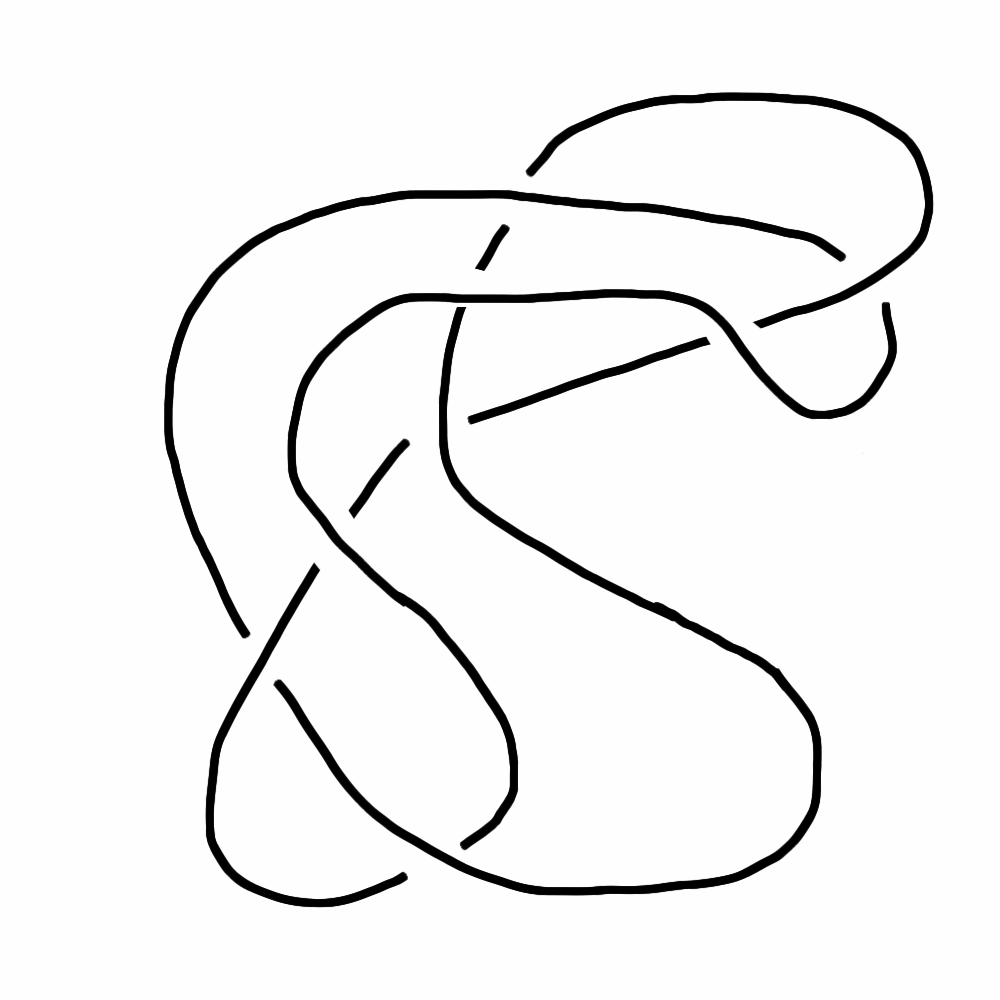
\includegraphics[width=\textwidth]{knotpics/anothersix-twisted.png}
                \caption{$6_1$ disguised}
        \end{subfigure}
\end{figure}

\begin{figure}[h]
        \centering
        \begin{subfigure}[b]{0.3\textwidth}
                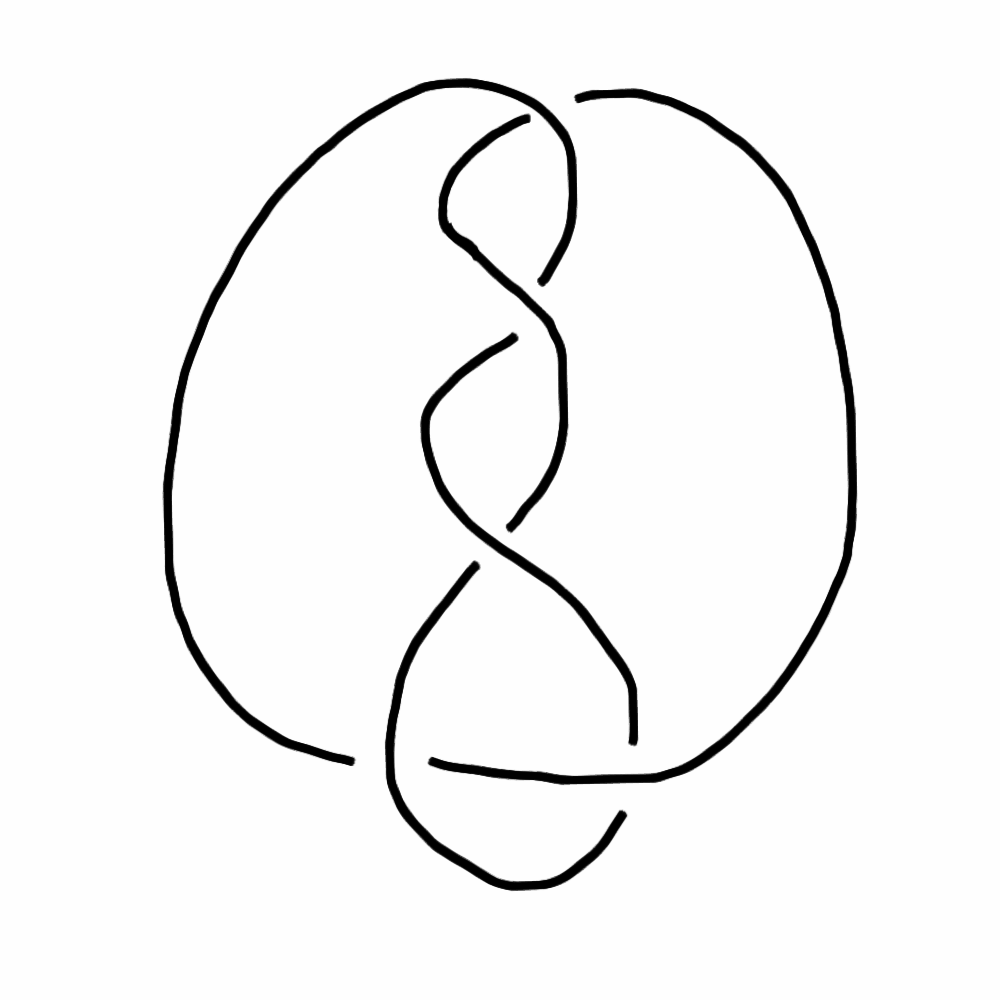
\includegraphics[width=\textwidth]{knotpics/sixcross.png}
                \caption{A five crossing knot}
        \end{subfigure}
        \begin{subfigure}[b]{0.3\textwidth}
                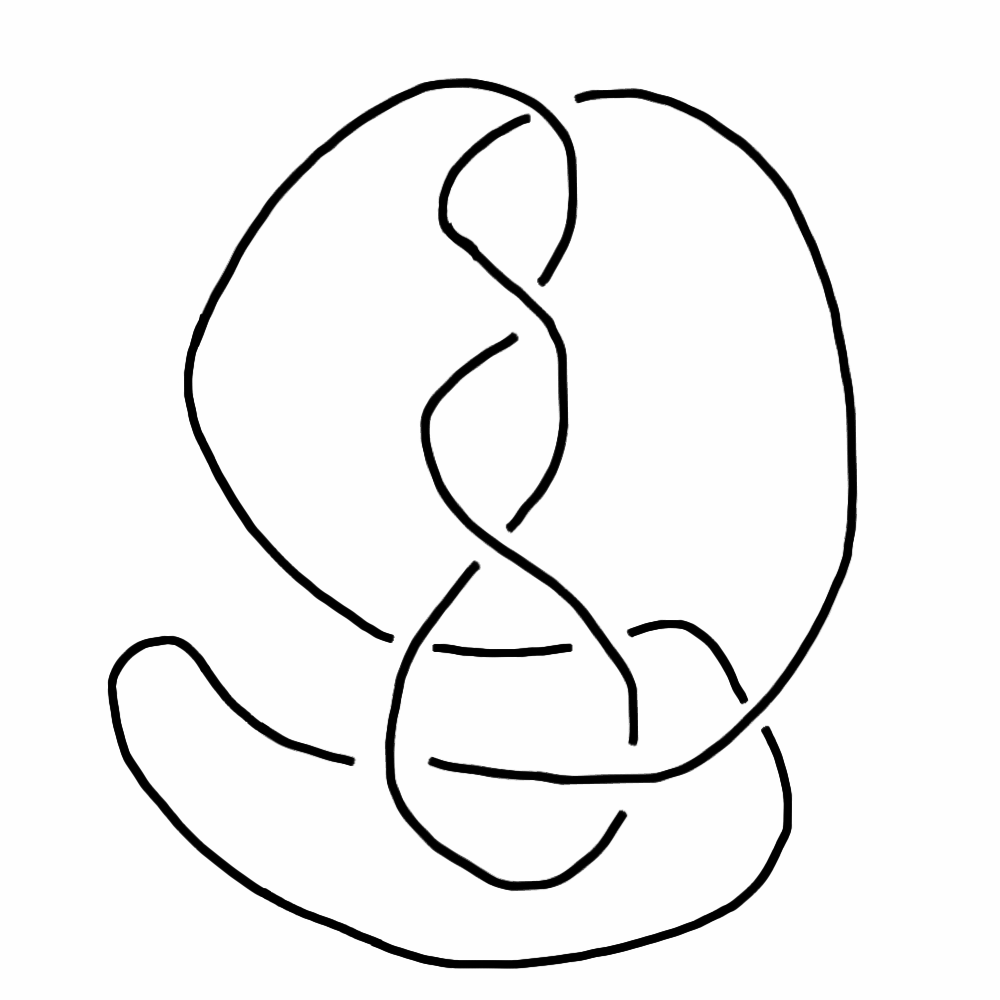
\includegraphics[width=\textwidth]{knotpics/sixcross-twistes.png}
                \caption{the same, disguised}
        \end{subfigure}
\end{figure}




\section*{Phase 2}
Ask them to use Reidemeister Moves to show a figure 8 knot is equivalent to its mirror image.

Draw the knots on the chalkboard. This facilitates the discussion.

\section*{Phase 3}
If there is time, ask them to work on the *nasty unkot* example from meeting 6 question 5. (This knot reappears in Assignment \#3.)

\section*{Announcment}
After class, send them a worked out version of a solution to the figure 8 knot problem.


\end{document}
%sagemathcloud={"zoom_width":100}